The first assumption that we address is that there are either zero or one targets to be localised. In many applications, this is an unrealistic assumption. For example, the ROCSAFE project which motivates this work, aims to apply object detection algorithms to aerial images in order to avoid the need to send a crime scene investigator into a hazardous scenario in order to verify the presence of a potential source of evidence \cite{Bagherzadeh2017ROCSAFE:Incidents}.\note{check the above sentence is consistent with the Background} An assumption that is more realistic is that there are a maximum of $K$ unknown sources present in the search region, which addresses the general case for the ROCSAFE \note{should ROCSAFE be in italics?} project.\par

\note{May need to go into more detail here since people without a background in probability might not understand implications of high-dimensional joint distribution}
The naive approach would be to introduce new random variables which represent the possible location of each target. Using the abbreviation T for target and Loc for location, this gives a set of random variables, whose joint distribution replaces that of TargetLocation: \[\{TOneLoc, TTwoLoc, TThreeLoc,...,TKLoc\}\] Each of these random variables has support $\{x_1, x_2, ..., x_N, x_{N+1}\}$, whereas before, $x_i$ represented the target location being at grid cell i for $i \in \{1,2, ..., N\}$ and $x_{N+1}$ represented that the target is not present. 
%This effectively extends the $TargetLocation$ variable used up to now to include the possibility of multiple targets being present. 
Assuming that targets cannot occupy the same grid cell, the update rule can be modified to assign the probability of the estimated state to be zero in the case that two target locations coincide. For example:
\footnotesize{
\[p(TOneLoc = x, TTwo = x, ..., TKLoc, SearchStatus, AgentLocation | SensorReading_{1:t}, Action_{1:t}) = 0\]}

\normalsize
Otherwise the update rule would be slightly modified to reflect the possibility of multiple targets: 


%\begin{figure}[H]
\scriptsize

\begin{gather}\label{eqn:JointTargetDistUpdate}
    \begin{split}
    %\centering
    p(SensorReading_t | AgentLoc_{t}, TOneLoc_{t}, ..., TKLoc_{t})  = 
    \\
    \begin{cases}
    \alpha \quad \text{ if } SensorReading_t=1 \text{ and } AgentLoc_t \neq TOneLoc_t \text{ and } AgentLoc_t \neq TTwoLoc_t \text{ and } ... \text{ and } AgentLoc_t \neq TKLoc_t
    \\
    1-\beta \quad \text{ if } SensorReading_t=1 \text{ and } \{ 
    TOneLoc_{t} = AgentLoc_{t} \text{ or } 
    TTwoLoc_{t} = AgentLoc_{t} \text{ or }...\text{ or }
    TKLoc_{t} = AgentLoc_{t}
    \}
    \\
    \beta \quad \text{ if } SensorReading_t=0 \text{ and } 
    \{
    TOneLoc_t = AgentLoc_t
    \text{ or } 
    TTwoLoc_t = AgentLoc_t
    \text{ or }...\text{ or }
    TKLoc_t = AgentLoc_t
    \}
    \\
    1-\alpha \quad \text{ if } SensorReading_t=0 \text{ and } 
    TOneLoc_t \neq AgentLoc_t
    \text{ and }
    TTwoLoc_t \neq AgentLoc_t
    \text{ and }...\text{ and }
    TKLoc_t \neq AgentLoc_t
    \end{cases}
    \end{split}
\end{gather}
\begin{center}
\small
Modifications to update rule for joint distribution accounting for multiple targets.
\end{center}
%\end{figure}

\normalsize

The main issue that arises using this approach is that there is an exponential increase the dimensionality of the hidden state for each new target added. This means that maintaining an estimate of the state quickly becomes infeasible, since the run time of the forward algorithm detailed in Section \ref{subsubsec:filteringDBN} is dependent on the square of the size of the joint distribution of the hidden state variables, $X_t$ and the memory requirements for maintaining the estimated state also depends on the dimensionality of the joint distribution of the hidden state. Therefore this naive approach is not feasible to implement in practice and other methods must be considered.
%See section \ref{subsubsec:filteringDBN} for details of the filtering algorithm.


Section \ref{sec:StochasticTargetLocalisationRelatedLiterature} of the literature review outlines a number of techniques that have been applied by other researchers in this domain in order to deal with the case of multiple targets which avoids the problem of creating an exponential increase in the size of the state. 
%\note{maybe should leave all of this to lit. review and just outline what I did.}
\citeauthor{Waharte2009CoordinatedUAVs} \cite{Waharte2009CoordinatedUAVs} describe an approach commonly used with occupancy grids, which is that every grid cell may or may not contain a target, independent of whether or not all other grid cells contain a target. When the location of the agent is known, this technique is often referred to as \textit{mapping}. This is described in the general case by \citeauthor{Thrun:2005:ProbabilisticRobotics} in  \cite[P.~284]{Thrun:2005:ProbabilisticRobotics}. Rather than maintaining a distribution representing the location of the single target, $TargetLocation$, as was the case in the work outlined up to this point in this chapter, we could create new binary random variables representing a target being present or not in each grid cell, denoted $m_i$ for $i \in \{1,..., N\}$, where $N$ is equal to the number of grid cells. $m$ is the joint distribution of these random variables. The DBN that would correspond to this is shown in Figure \ref{fig:DBNWithMultipleIndependent}. The agent maintains the estimate of the map: \[p(m | SensorReading_{1:t}, Action_{1:t}) = \prod\limits_{i}p(m_i | SensorReading_{1:t}, Action_{1:t})\]

%The estimated state of each grid cell, $m_i$, is maintained by the agent. 
The update rule simply updates only the estimated state of the grid cell at which the reading was taken, as outlined in \cite{Waharte2009CoordinatedUAVs}.

\begin{figure}[h]
    \centering
    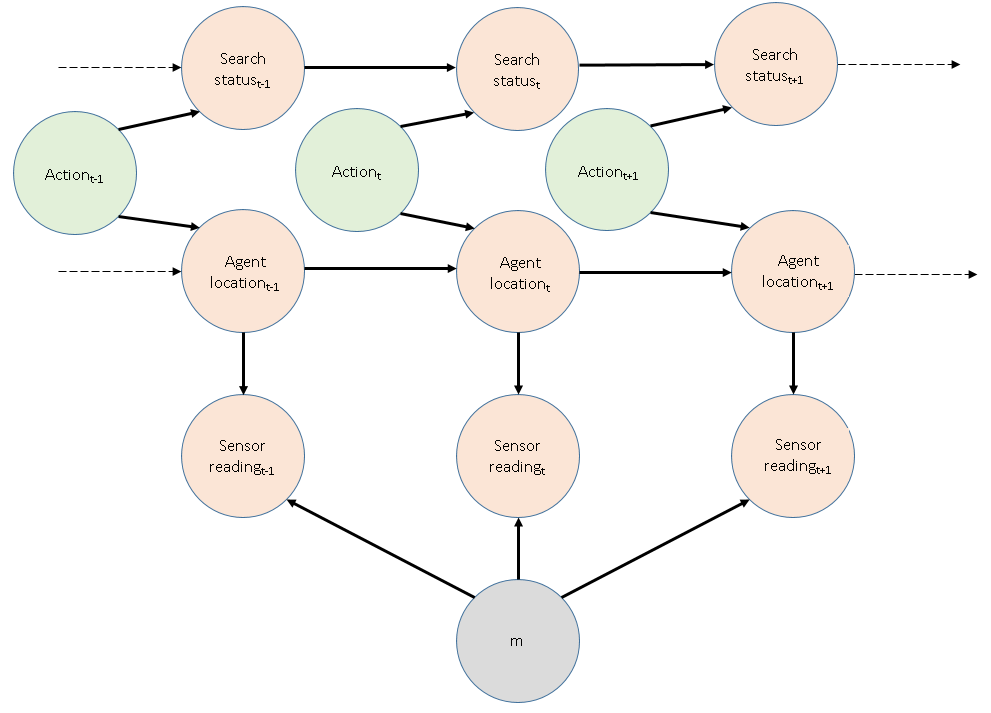
\includegraphics[width = 0.86\linewidth]{Chapters/MultiAgentTargetDetection/Figs/DBNs/DBNWithMultipleIndependentSources.png}
    \caption{The DBN which takes into account that there could be a target in each of the grid cells}
    \label{fig:DBNWithMultipleIndependent}
\end{figure}

%In the case, estimating the joint distribution is not hard, since This results in a greatly simplified state estimate update equation, where the probability of the target being located in a grid cell does not change unless the observation was made in that grid cell.
The major drawback of this approach is that there is no clear way to apply the SPRT, which meant that our implementation for this approach required a new method for terminating the search.
%hence an alternative method of terminating the search is required.
Instead, we chose to use a simple extension to the approach proposed in this chapter in the sections prior to this one.
%We took inspiration from the way that searching for multiple targets would intuitively be carried out: we keep searching for another target until we are "satisfied" that we have enough information to conclude there are no more targets left to find.
We chose to run a sequential search, which locates sources one-by-one, using information from the previous search to begin the subsequent search for the next target. This uses the advantages of using the sequential search procedure with the SPRT while avoiding the dimensionality problems that arise with introducing extra targets that would arise from a simultaneously searching for multiple targets. The search procedure we propose for multiple sources is given in Algorithm \ref{alg:MultiTargetLocalisation}. 
\begin{algorithm}[H]
\caption{Multiple Target Localisation Algorithm}
\label{alg:MultiTargetLocalisation}

\begin{algorithmic}[1]
\renewcommand{\algorithmicrequire}{\textbf{Input:}}
\renewcommand{\algorithmicensure}{\textbf{Output:}}
%Input
\REQUIRE $ \newline initial\_est\_state = p(x_{0} | e_{0}, u_0)=bel(x_{0}): \quad\text{ The initial estimated state distribution}
\newline K: \quad \text{ The maximum number of targets to be localised.}
\newline find\_next\_target: \quad \text{ The procedure for locating targets described in Algorithm \ref{alg:SingleTargetLocalisation}}$
%Output
\ENSURE $\newline \text{A set of target locations, of size }\leq \text{ K}$

\hfill\pagebreak
\STATE target\_locations $\leftarrow$ empty array
\STATE estimated\_state $\leftarrow$ initial\_est\_state
\WHILE{target\_locations.length $\leq$ K}
\STATE next\_target\_location $\leftarrow$ find\_next\_target(estimated\_state)
\IF{next\_target is $x_{N+1}$}
\STATE {break}
\ELSE 
\STATE{target\_locations.append(next\_target\_location)}
\STATE{Update the estimated\_state probability where (target\_location = next\_target\_location) to zero}
\STATE{Normalize the estimated state probabilities to sum to one}
\ENDIF
\ENDWHILE

\RETURN target\_locations
\end{algorithmic} 
\end{algorithm}
\normalsize
The algorithm maintains a list of located targets in the variable $target\_locations$ and runs the $find\_next\_target$ procedure until the SPRT returns that there is no target present using the most recent state estimate. Lines 9 and 10 effectively restart the search procedure for a single source with the probability at the location where the last target was located set to zero. This means that it will continue to be zero, due to the multiplicative update formula, which effectively removes it from the process of localising subsequent targets. This allows us to extend the framework developed for the search procedure so far, which greatly simplifies the process of writing the implementation code to perform the search and the subsequent analysis of results.

%\note{Talk about how prior can be specified to guide search to certain regions before others - Maybe this should be in conclusion/discussion section?}
%Taking advantage of the fact that our representations  This is best described in algorithm
